% VLDB template version of 2020-08-03 enhances the ACM template, version 1.7.0:
% https://www.acm.org/publications/proceedings-template
% The ACM Latex guide provides further information about the ACM template

\documentclass[sigconf, nonacm]{acmart}

%% The following content must be adapted for the final version
% paper-specific
\newcommand\vldbdoi{XX.XX/XXX.XX}
\newcommand\vldbpages{XXX-XXX}
% issue-specific
\newcommand\vldbvolume{14}
\newcommand\vldbissue{1}
\newcommand\vldbyear{2020}
% should be fine as it is
\newcommand\vldbauthors{\authors}
\newcommand\vldbtitle{\shorttitle} 
% leave empty if no availability url should be set
\newcommand\vldbavailabilityurl{https://github.com/mirzaim/VisionGNN}
% whether page numbers should be shown or not, use 'plain' for review versions, 'empty' for camera ready
\newcommand\vldbpagestyle{plain}

\usepackage{algorithm}
\usepackage{algorithmic}

\usepackage{multirow}
\usepackage{pifont}

\newcommand{\cmark}{\ding{51}}
\newcommand{\xmark}{\ding{55}}

\begin{document}
\title{Vision Graph Neural Networks: A Replication Study}

%%
%% The "author" command and its associated commands are used to define the authors and their affiliations.
\author{Morteza Mirzaei}
\affiliation{%
  \institution{McMaster University}
  \city{Hamilton}
  \state{Ontario}
  \country{Canada}
}
\email{mirzam48@mcmaster.ca}

%%
%% The abstract is a short summary of the work to be presented in the
%% article.
\begin{abstract}
  This paper aims to implement and replicate the findings of the Vision Graph Neural Networks (ViG) paper. ViG adopts a novel approach by treating images as graphs and utilizing graph neural networks (GNNs) algorithms for feature extraction and downstream tasks. We will reproduce experiments and conduct ablation studies to evaluate ViG's performance in tasks such as image classification, thus contributing to the assessment of its reproducibility and potential in visual perception tasks. Additionally, we will discuss challenges encountered during implementation, such as missing details or implementation complexities. The code for our implementation can be accessed at \url{https://github.com/mirzaim/VisionGNN}.
\end{abstract}

\maketitle

% %%% do not modify the following VLDB block %%
% %%% VLDB block start %%%
% \pagestyle{\vldbpagestyle}
% \begingroup\small\noindent\raggedright\textbf{PVLDB Reference Format:}\\
% \vldbauthors. \vldbtitle. PVLDB, \vldbvolume(\vldbissue): \vldbpages, \vldbyear.\\
% \href{https://doi.org/\vldbdoi}{doi:\vldbdoi}
% \endgroup
% \begingroup
% \renewcommand\thefootnote{}\footnote{\noindent
%   This work is licensed under the Creative Commons BY-NC-ND 4.0 International License. Visit \url{https://creativecommons.org/licenses/by-nc-nd/4.0/} to view a copy of this license. For any use beyond those covered by this license, obtain permission by emailing \href{mailto:info@vldb.org}{info@vldb.org}. Copyright is held by the owner/author(s). Publication rights licensed to the VLDB Endowment. \\
%   \raggedright Proceedings of the VLDB Endowment, Vol. \vldbvolume, No. \vldbissue\ %
%   ISSN 2150-8097. \\
%   \href{https://doi.org/\vldbdoi}{doi:\vldbdoi} \\
% }\addtocounter{footnote}{-1}\endgroup
% %%% VLDB block end %%%

% %%% do not modify the following VLDB block %%
% %%% VLDB block start %%%
% \ifdefempty{\vldbavailabilityurl}{}{
%   \vspace{.3cm}
%   \begingroup\small\noindent\raggedright\textbf{PVLDB Artifact Availability:}\\
%   The source code, data, and/or other artifacts have been made available at \url{\vldbavailabilityurl}.
%   \endgroup
% }
% %%% VLDB block end %%%

\section{Introduction}

Traditional convolutional neural networks (CNNs) have historically dominated the landscape of computer vision. However, recent advancements in transformer architectures \cite{attentionisallyouneed, ViT}, coupled with attention mechanisms, have propelled Vision Graph Neural Networks (ViG) \cite{visiongnn} into the spotlight. By treating images as graphs and harnessing the power of graph neural networks (GNNs), ViG offers more adaptability and efficacy in visual perception tasks, transcending the limitations of conventional grid or sequence representations. The seminal Vision GNN paper \cite{visiongnn} introduces an innovative architecture that partitions input images into patches, each treated as a node within a graph. Through iterative information exchange among these nodes via graph convolutional and feed-forward network modules, ViG achieves remarkable performance across diverse tasks such as image classification and object detection.

In this paper, we aim to replicate the results of the Vision GNN paper \cite{visiongnn}. Our methodology involves a comprehensive discussion of the datasets and experimental setups employed for our investigations. We replicate the experiments conducted in the original paper, including the main results and ablation studies on architecture. Furthermore, we delve into the challenges encountered during the implementation process and elucidate the strategies employed to overcome them. Through our endeavors, we seek to contribute to the examination of the reproducibility of the ViG model.

\section{Experiments}
In this section, we conduct experiments to demonstrate the effectiveness of ViG models with image classification tasks. We begin by outlining the datasets used for training and evaluation, followed by details of the experimental setup, including model configurations and training procedures.
% Subsequently, we present and analyze the experimental results to assess the performance of ViG models across various benchmarks and compare them with baseline approaches.

\begin{table*}[t]
  \setlength{\tabcolsep}{12pt}
  \caption{Results of VisionGNN models on Imagenette and Imagewoof datasets.}
  \label{tab:results}
  \begin{tabular}{cccccc}
    \toprule
    \multirow{2}{*}{Model} & \multirow{2}{*}{Depth} & \multirow{2}{*}{Dimension} & \multirow{2}{*}{Params (M)} & \multicolumn{2}{c}{Top-1 Accuracy}             \\
                           &                        &                            &                             & Imagenette                         & Imagewoof \\
    \midrule
    VisionGNN-Tiny  & 12   & 192    & 9.8     & 69.04      & 42.61     \\
    VisionGNN-Small & 16   & 320    & 36.2    & 72.36      & 45.00     \\
    VisionGNN-Big   & 16   & 640    & 144.5   & 74.39      & 45.97     \\
    \bottomrule
  \end{tabular}
\end{table*}


\begin{figure}[t]
  \centering
  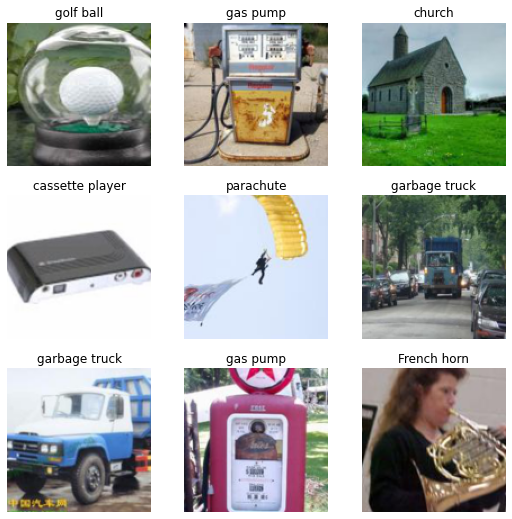
\includegraphics[width=0.9\linewidth]{figures/imagenette.png}
  \caption{Sample images from the Imagenette dataset.}
  \label{fig:imagenette}
\end{figure}

\subsection{Datasets}

We utilized two smaller datasets compared to ImageNet \cite{imagenet} in our experiments: the Imagenette dataset and the Imagewoof dataset \cite{imagenette}, due to limited resources.

The Imagenette dataset is a subset of 10 classified classes from ImageNet, featuring diverse categories such as tench, English springer, cassette player, chain saw, church, French horn, garbage truck, gas pump, golf ball, and parachute (see Figure \ref{fig:imagenette}). The Imagenette dataset is publicly available on GitHub at the following link: \url{https://github.com/fastai/imagenette}. It comprises 13,394 images, with a 70/30 train/validation split.

Similarly, we employed the Imagewoof dataset, a subset of 10 dog breeds from ImageNet that present more challenging classification tasks. The included breeds are Australian terrier, Border terrier, Samoyed, Beagle, Shih-Tzu, English foxhound, Rhodesian ridgeback, Dingo, Golden retriever, and Old English sheepdog. The Imagewoof dataset contains 12,954 images with 70/30 train/validation split. It is accessible through the same GitHub repository as Imagenette.

For consistency and computational efficiency, we utilized the '320 px' version of both datasets, where images have their shortest side resized to 320 pixels while maintaining aspect ratio. This version ensures standardized resolution across the dataset, facilitating uniformity in image dimensions for both training and evaluation purposes.

To facilitate reproducibility and ease of access, we provide a script named \texttt{get\_dataset.sh} within our code repository. This script automates the process of downloading and extracting both the Imagenette and Imagewoof datasets to the appropriate location, ensuring consistency across different environments and simplifying the setup process for reproducing our experiments.

\subsection{Experimental Settings}
We employed the GELU activation function \cite{gelus} within our neural network architecture, resizing each image to dimensions of $224 \times 224$. Data augmentation techniques included Random Augmentation \cite{randaugment}, Random Erasing \cite{randerase}, and Horizontal Flip. Prior to training, images were normalized using the mean and standard deviation from the ImageNet dataset \cite{imagenet}. Although initial experiments with Mixup \cite{mixup} and Cutmix \cite{cutmix} augmentation did not yield significant improvements, subsequent research suggested their efficacy in higher epochs, typically beyond 80 \cite{mixup_without_hesitation, mixup_overtraining}. Because of limited resources and time, we trained the model for 80 epochs; therefore, Mixup and Cutmix were not utilized in the final training. A batch size of 64 images was utilized for training, with a classifier comprising two linear layers with dimensions of $\text{input features} \rightarrow 1024 \rightarrow \text{number of classes}$. Loss optimization was performed using the Cross-Entropy loss function, coupled with the Adam optimizer \cite{adamoptimizer} with learning rate, $\beta_1$, and $\beta_2$ values set to $10^{-5}$, $0.9$, and $0.999$ respectively. Implementation of the model was conducted using the PyTorch framework \cite{pytorch}. Notably, computational resources utilized for training comprised an Intel Core i9-13900KF CPU, 32 GB RAM, and an NVIDIA GeForce RTX 4090 GPU with 24 GB dedicated memory.

\begin{table}[b]
  % \setlength{\tabcolsep}{12pt}
  \caption{Ablation study of different modules in VisionGNN.}
  \label{tab:abl_modules}
  \begin{tabular}{ccccc}
    \toprule
    GraphConv & FC in Grapher        & FFN        & Params (M) & Top-1 Acc      \\
    \midrule
    \cmark    & \xmark               & \xmark     & 3.2        & 71.80          \\
    \cmark    & \cmark               & \xmark     & 9.8        & 73.10          \\
    \cmark    & \xmark               & \cmark     & 29.6       & 74.83          \\
    \cmark    & \cmark               & \cmark     & 36.2       & 72.36          \\
    \bottomrule
  \end{tabular}
\end{table}

\subsection{Main Results}

In this section, we present the performance analysis of VisionGNN models on the Imagenette and Imagewoof datasets. The main paper discusses two implementations of VisionGNN: Isotropic and Pyramid. For this study, we focused on the Isotropic architecture, which maintains the feature size unchanged in its main computational body, facilitating scalability and hardware acceleration. This architectural scheme has gained popularity in transformer models for natural language processing \cite{attentionisallyouneed}, and recent advancements in vision-based neural networks have also explored its efficacy, such as MLP-Mixer \cite{mlpmixer}, ViT \cite{ViT}, and ResMLP \cite{resmlp}.

Table \ref{tab:results} provides an overview of the results obtained for VisionGNN models of varying sizes. All models were trained for 80 epochs, although it should be noted that the largest network could potentially benefit from additional training epochs as it was still converging. However, due to constraints in time and resources, training was terminated at 80 epochs. The table illustrates the top-1 accuracy achieved by VisionGNN models on both Imagenette and Imagewoof datasets, demonstrating the performance of the Isotropic architecture across different network sizes. As you can see, by increasing the model size, the accuracy generally increases.

\begin{figure}[b]
  \centering
  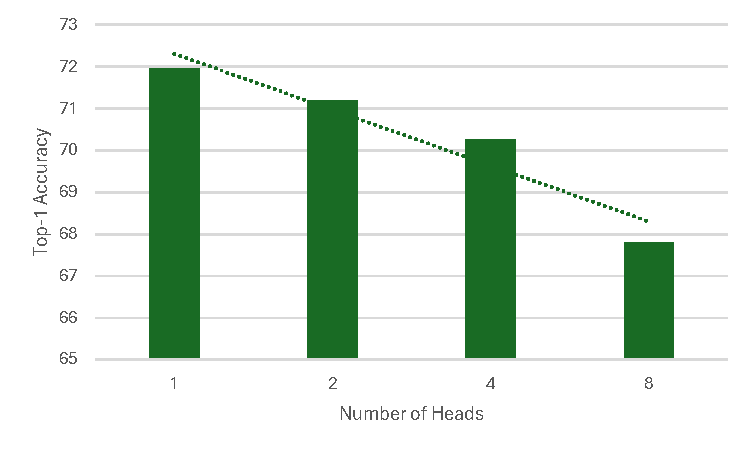
\includegraphics[width=\linewidth]{figures/num_head_chart.pdf}
  \caption{Effect of the number of heads on the top-1 accuracy of the VisionGNN model. The x-axis represents the number of heads, while the y-axis represents the top-1 accuracy achieved on the Imagenette dataset.}
  \label{fig:num_head_chart}
\end{figure}

\subsection{Ablation Study}
To further investigate the impact of different components within the VisionGNN architecture, we conducted an ablation study to assess the performance of the model under various conditions. We conduct ablation study of the proposed method on Imagenette classification task and use the isotropic VisionGNN-Small as the base architecture.

\subsubsection{The effect of different modules in VisionGNN}

To adapt the graph neural network to visual tasks, fully connected (FC) layers were introduced in the Grapher module, and feedforward neural network (FFN) blocks were utilized for feature transformation. The effects of these modules were evaluated through an ablation study. It's worth noting that all models were trained for 80 epochs, which may not have been sufficient for the model with all components to fully converge and optimize the FC layers. As a result, a performance degradation was observed in the last row of Table \ref{tab:abl_modules}. However, if training were to continue, it is expected that the accuracy of the model with all components would surpass that of the previous configurations.

\subsubsection{The number of heads} \label{sec:num_heads}

The multi-head update operation enables the Grapher module to process node features in different subspaces. The number of heads controls the transformation diversity in these subspaces. It's assumed that different subspaces are independent from each other. Therefore, increasing the number of heads results in fewer parameters overall, but it also diminishes the connections between different parts of the vector. As observed in Figure \ref{fig:num_head_chart}, the accuracy generally decreases with an increase in the number of heads. For the main model, we chose the number of heads equal to one as the default value.

\subsubsection{The number of neighbors}

The number of neighboring nodes during graph construction is a crucial parameter affecting the range of information aggregation. Striking a balance is essential, as too few neighbors hinder effective information exchange, while an excessive number may cause over-smoothing. We conducted experiments by varying the parameter \( K \) from 3 to 20 and present the results in Figure \ref{fig:num_neighbor_chart}. Our analysis reveals that optimal performance on the Imagenette classification task is observed when \( K \) is within the range of 12 to 15.

\begin{figure}[t]
  \centering
  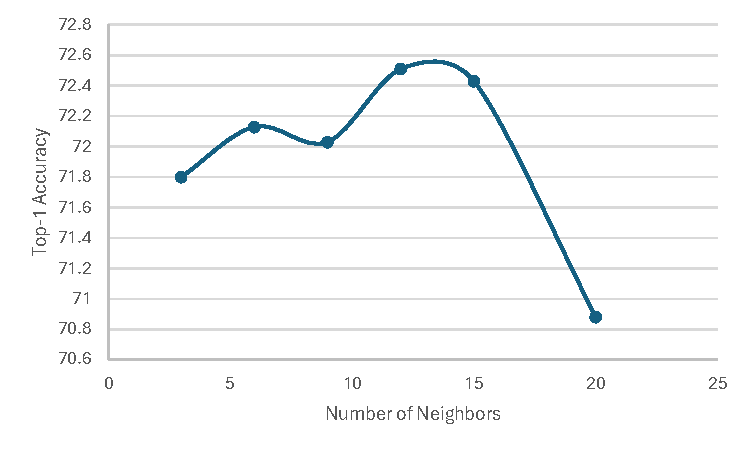
\includegraphics[width=\linewidth]{figures/num_neighbor_chart.pdf}
  \caption{Performance comparison of different numbers of neighbors on the Imagenette dataset. The chart illustrates the impact of varying the parameter \( K \) on the classification task accuracy.}
  \label{fig:num_neighbor_chart}
\end{figure}

\section{Reimplementation Challenges}
In this section, we discuss the challenges encountered during the reimplementation of the paper. Despite diligent efforts to reproduce the reported results, several obstacles were encountered along the way. We provide insights into these challenges and detail the strategies employed to overcome them, offering valuable lessons for future endeavors in replicating research findings.

\subsection{Graph Structure Extraction}
At the outset of the reimplementation process, a challenge arose from a misconception regarding the extraction of the graph structure from the image. Initially, it was inferred from the paper that a single graph structure should be extracted from the image at the beginning and maintained throughout the entirety of the model's architecture and higher layers. However, it became evident that, in reality, recalculating the graph structure was necessary at each layer of the model.

In different layers of the model, the level of detail or abstraction from the input data varies. Some layers focus on basic features like edges or shapes, while others focus on more complex patterns or concepts. When we try to preserve the same graph structure derived from the simpler features in the lower layers and use it in the higher layers, it doesn't work well. This is because, in the higher layers where the model deals with more abstract concepts, it needs to make connections between distant features or elements in the input data. So, the graph structure needs to adapt and change at each layer to accommodate these long-distance connections. The architecture is more like a transformer, and each layer needs to find different graph connections.

\subsection{Effectiveness of Mixup and Cutmix}
\begin{figure}[t]
  \centering
  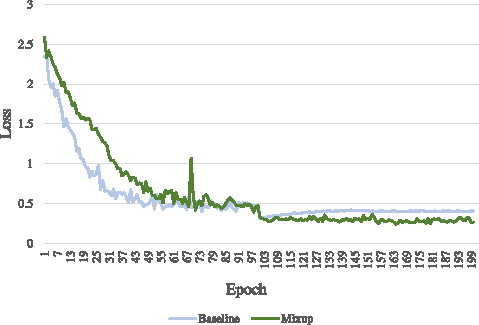
\includegraphics[width=0.9\linewidth]{figures/mixup_training.pdf}
  \caption{Training loss comparison with and without Mixup augmentation. The figure is adapted from \cite{mixupwithouthesitation}.}
  \label{fig:mixup_training}
\end{figure}

Another challenge emerged when attempting to utilize advanced data augmentation techniques such as Mixup \cite{mixup} and Cutmix \cite{cutmix}. Despite experimenting with various hyperparameters, these augmentation methods resulted in decreased model accuracy. Upon investigation, it was discovered that these techniques require longer training durations to become effective. Specifically, it was observed that Mixup, a commonly used augmentation method, necessitates more epochs to converge due to its exploration of additional regions in the data space. For instance, while a standard training routine of 90 epochs may suffice, training ResNet-50 on ImageNet with Mixup typically requires up to 200 epochs to achieve convergence. This phenomenon extends beyond Mixup and is also observed in other augmentation methods, which significantly enhance the complexity of training data \cite{cutmix, gridmask}.

An analysis of the training loss for ResNet-18 with and without Mixup augmentation revealed an intriguing pattern visualized in figure \ref{fig:mixup_training}. Initially, the loss was higher with Mixup, particularly in the early epochs. However, beyond 100 epochs, the loss consistently decreased with Mixup, lowering the training loss without augmentation \cite{mixupwithouthesitation}.

Although the benefits of these augmentation techniques become apparent after a certain number of epochs, our constrained resources and time limitations prevented us from fully exploiting their potential. Consequently, Mixup and Cutmix augmentations were not incorporated into the final training process.

\subsection{Feature Extraction from Patches}
The original paper does not provide details on how to extract features from patches. In our reimplementation, we utilized a method involving six linear layers to extract features, where each patch is flattened and fed into the network. Each layer consists of a fully connected neural network, batch normalization layer, and GELU activation function. This architecture resembles an autoencoder. A diagram of the network can be seen in Figure \ref{fig:feature_extractor_arch}.

\begin{figure}[t]
  \centering
  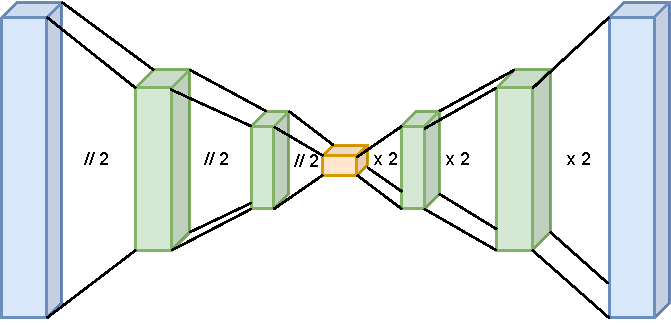
\includegraphics[width=0.9\linewidth]{figures/feature_extractor_arch.pdf}
  \caption{rchitecture of the feature extractor used in our reimplementation.}
  \label{fig:feature_extractor_arch}
\end{figure}

Upon further investigation and examination of other implementations of the paper, we discovered that the original approach utilizes a more advanced method known as overlapping feature extraction. This method involves an overlapping sliding window into one token progressively (see Figure \ref{fig:overlapping_nonoverlapping}) and employing a deep convolutional neural network to extract features \cite{pvtv2}. Even though the overlapping feature extraction method is more advanced and computationally expensive, our method is simpler and able to achieve similar results.

\subsection{Distance Measure in KNN Calculation}
The original paper does not specify how they measure the distance between feature vectors when calculating K-nearest neighbors (KNN). In our reimplementation, for simplicity, we opted to use cosine similarity, which involves taking the inner product of two vectors and selecting the $k$ most similar ones as the output of the KNN algorithm.

Upon reviewing the original paper's code, it appears that they employ a more advanced KNN algorithm known as "Dilated KNN." This method utilizes the Dilated $k$-NN to find dilated neighbors after every Graph Convolutional Network (GCN) layer and construct a Dilated Graph. Specifically, for an input graph $\mathcal{G}=(\mathcal{V}, \mathcal{E})$ with Dilated $k$-NN and $d$ as the dilation rate, the Dilated $k$-NN returns the $k$ nearest neighbors within the $k\times d$ neighborhood region by skipping every $d$ neighbors. The nearest neighbors are determined based on a pre-defined distance metric, commonly the $\ell_2$ distance in the feature space of the current layer \cite{deepgcns}.

Despite the advanced nature of Dilated KNN, our approach using cosine similarity proved to be more computationally efficient while achieving comparable accuracy.

\begin{figure}[t]
  \centering
  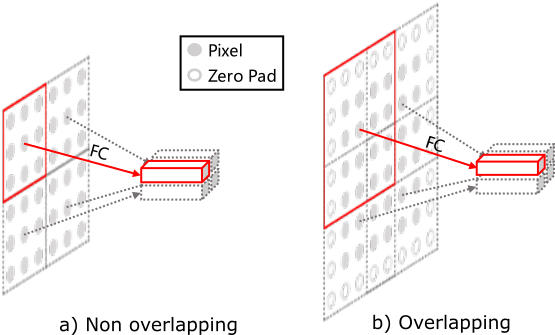
\includegraphics[width=0.9\linewidth]{figures/overlapping_nonoverlapping.png}
  \caption{Comparison between overlapping and non-overlapping feature extraction methods. This figure is adapted from \cite{pvtv2}.}
  \label{fig:overlapping_nonoverlapping}
\end{figure}

\subsection{Multi-Head layer implementation}
As we explained in the \ref{sec:num_heads}, we devide the feature space to subspaces as number of heads and apply the different transformation to each subspace and then concatenate the results. In the first, implementation we used number of heads time the linear layer to apply the transformation to each subspace and concatenate the results. However, as the number of heads increases, this implementation becomes inefficient and computationally expensive because it uses the for loop to apply the transformation to each subspace as you can see in Algorithm \ref{alg:linear_layers}.

But we find out we could use 1d convolutional layer with kernel size of one and group size of number of heads. This layer is equivalent to the linear layer for each subspace and concatenation of the results. This implementation fully utilizes the parallel processing capabilities of the GPU and more efficient in maner of time and memory.

\begin{algorithm}
  \caption{Multi-Head Layer Implementation with Linear Layers}
  \label{alg:linear_layers}
  \begin{algorithmic}[1]
    \STATE \textbf{Input:} Input vectors $V$, number of heads $h$
    \STATE \textbf{Output:} Transformed vectors $\tilde{V}$
    \STATE Divide input vectors into $h$ heads: $v_1, \ldots, v_h := V$
    \FOR{$i = 1$ \TO $h$}
    \STATE $\tilde{v}_i = W_i \cdot v_i + b_i$
    \ENDFOR
    \STATE $\tilde{V} = \text{concatenate}([\tilde{v}_1, \ldots, \tilde{v}_h])$
  \end{algorithmic}
\end{algorithm}

\clearpage

\bibliographystyle{ACM-Reference-Format}
\bibliography{main}

\end{document}
\endinput
